\documentclass[xcolor=pdflatex,dvipsnames,table]{beamer}
\usepackage{epsfig,graphicx}
\usepackage{palatino}
\usepackage{fancybox}
\usepackage{relsize}
\usepackage[procnames]{listings}

% "define" Scala
\usepackage[T1]{fontenc}  
\usepackage[scaled=0.82]{beramono}  
\usepackage{microtype} 

\sbox0{\small\ttfamily A}
\edef\mybasewidth{\the\wd0 }

\lstdefinelanguage{scala}{
  morekeywords={abstract,case,catch,class,def,%
    do,else,extends,false,final,finally,%
    for,if,implicit,import,match,mixin,%
    new,null,object,override,package,%
    private,protected,requires,return,sealed,%
    super,this,throw,trait,true,try,%
    type,val,var,while,with,yield},
  sensitive=true,
  morecomment=[l]{//},
  morecomment=[n]{/*}{*/},
  morestring=[b]",
  morestring=[b]',
  morestring=[b]"""
}

\usepackage{color}
\definecolor{dkgreen}{rgb}{0,0.6,0}
\definecolor{gray}{rgb}{0.5,0.5,0.5}
\definecolor{mauve}{rgb}{0.58,0,0.82}

% Default settings for code listings
\lstset{language=scala,
  showstringspaces=false,
  columns=fixed, % basewidth=\mybasewidth,
  basicstyle={\small\ttfamily},
  numbers=none,
  numberstyle=\footnotesize\color{gray},
  % identifierstyle=\color{red},
  keywordstyle=\color{blue},
  commentstyle=\color{dkgreen},
  stringstyle=\color{mauve},
  breakatwhitespace=true,
  procnamekeys={def, val, var, class, trait, object, extends},
  procnamestyle=\ttfamily\color{red},
}

\lstnewenvironment{scala}
{\lstset{language=scala}}
{}
\lstnewenvironment{cpp}
{\lstset{language=C++}}
{}
\lstnewenvironment{bash}
{\lstset{language=bash}}
{}
\lstnewenvironment{verilog}
{\lstset{language=verilog}}
{}

\newcommand{\isc}{
\lstinline
}

\lstdefinestyle{scala}{language=scala,
  showstringspaces=false,
  columns=fixed, % basewidth=\mybasewidth,
  basicstyle={\small\ttfamily},
  numbers=none,
  numberstyle=\footnotesize\color{gray},
  % identifierstyle=\color{red},
  keywordstyle=\color{blue},
  commentstyle=\color{dkgreen},
  stringstyle=\color{mauve},
  breakatwhitespace=true,
  procnamekeys={def, val, var, class, trait, object, extends},
  procnamestyle=\ttfamily\color{red},
}

\lstset{basicstyle={\footnotesize\ttfamily}}

\usetheme[height=8mm]{Rochester}
\setbeamersize{text margin left=3mm} 
\setbeamersize{text margin right=3mm} 
\setbeamertemplate{navigation symbols}{}

\definecolor{Cobalt}{rgb}{0.25,0.125,0.70}
\definecolor{RedOrange}{rgb}{0.8,0.25,0.0}
% \definecolor{RedOrange}{rgb}{0.8,0.775,0.25}
\def\frametitledefaultcolor{Cobalt}
\def\frametitleproblemcolor{RedOrange}

\lstset{basicstyle={\footnotesize\ttfamily}}

\setbeamertemplate{frametitle}
{
\vskip-7mm
\textbf{\insertframetitle}\hfill\insertframenumber
}
\setbeamercolor{frametitle}{bg=\frametitledefaultcolor}

\newenvironment{sample}{\VerbatimEnvironment\begin{footnotesize}\begin{semiverbatim}}{\end{semiverbatim}\end{footnotesize}}

\newenvironment{FramedSemiVerb}%
{\begin{Sbox}\begin{minipage}{.94\textwidth}\begin{semiverbatim}}%
{\end{semiverbatim}\end{minipage}\end{Sbox}
\setlength{\fboxsep}{8pt}\fbox{\TheSbox}}

\newenvironment{FramedVerb}%
{\VerbatimEnvironment
\begin{Sbox}\begin{minipage}{.94\textwidth}\begin{Verbatim}}%
{\end{Verbatim}\end{minipage}\end{Sbox}
\setlength{\fboxsep}{8pt}\fbox{\TheSbox}}

% \newenvironment{sample}{\VerbatimEnvironment\begin{footnotesize}\begin{Verbatim}}{\end{Verbatim}\end{footnotesize}}
\newcommand{\code}[1]{\begin{footnotesize}{\tt #1}\end{footnotesize}}
\newcommand{\comment}[1]{{\color{Green}\it\smaller #1}}


\title{Chisel @ CS250 -- Part III -- Lecture 8}
\author{Jonathan Bachrach}
\date{\today}
\institute[UC Berkeley]{EECS UC Berkeley}

\begin{document}

\begin{frame}
\titlepage
\end{frame}
\addtocounter{framenumber}{-1}

\begin{frame}{Options for Testing Chisel Designs}
\begin{itemize}
\item testing using assert and printf in Chisel
\item testing Verilog using VCS
\item testing from within Scala
\begin{itemize}
\item test C++ executable
\item test Verilog using VCS
\end{itemize}
\item testing inside C++ simulator
\begin{itemize}
\item VCD debugging
\item manual testing from within C++
\end{itemize}
\end{itemize}
\end{frame}

\begin{frame}{Simulation Options}
\begin{center}
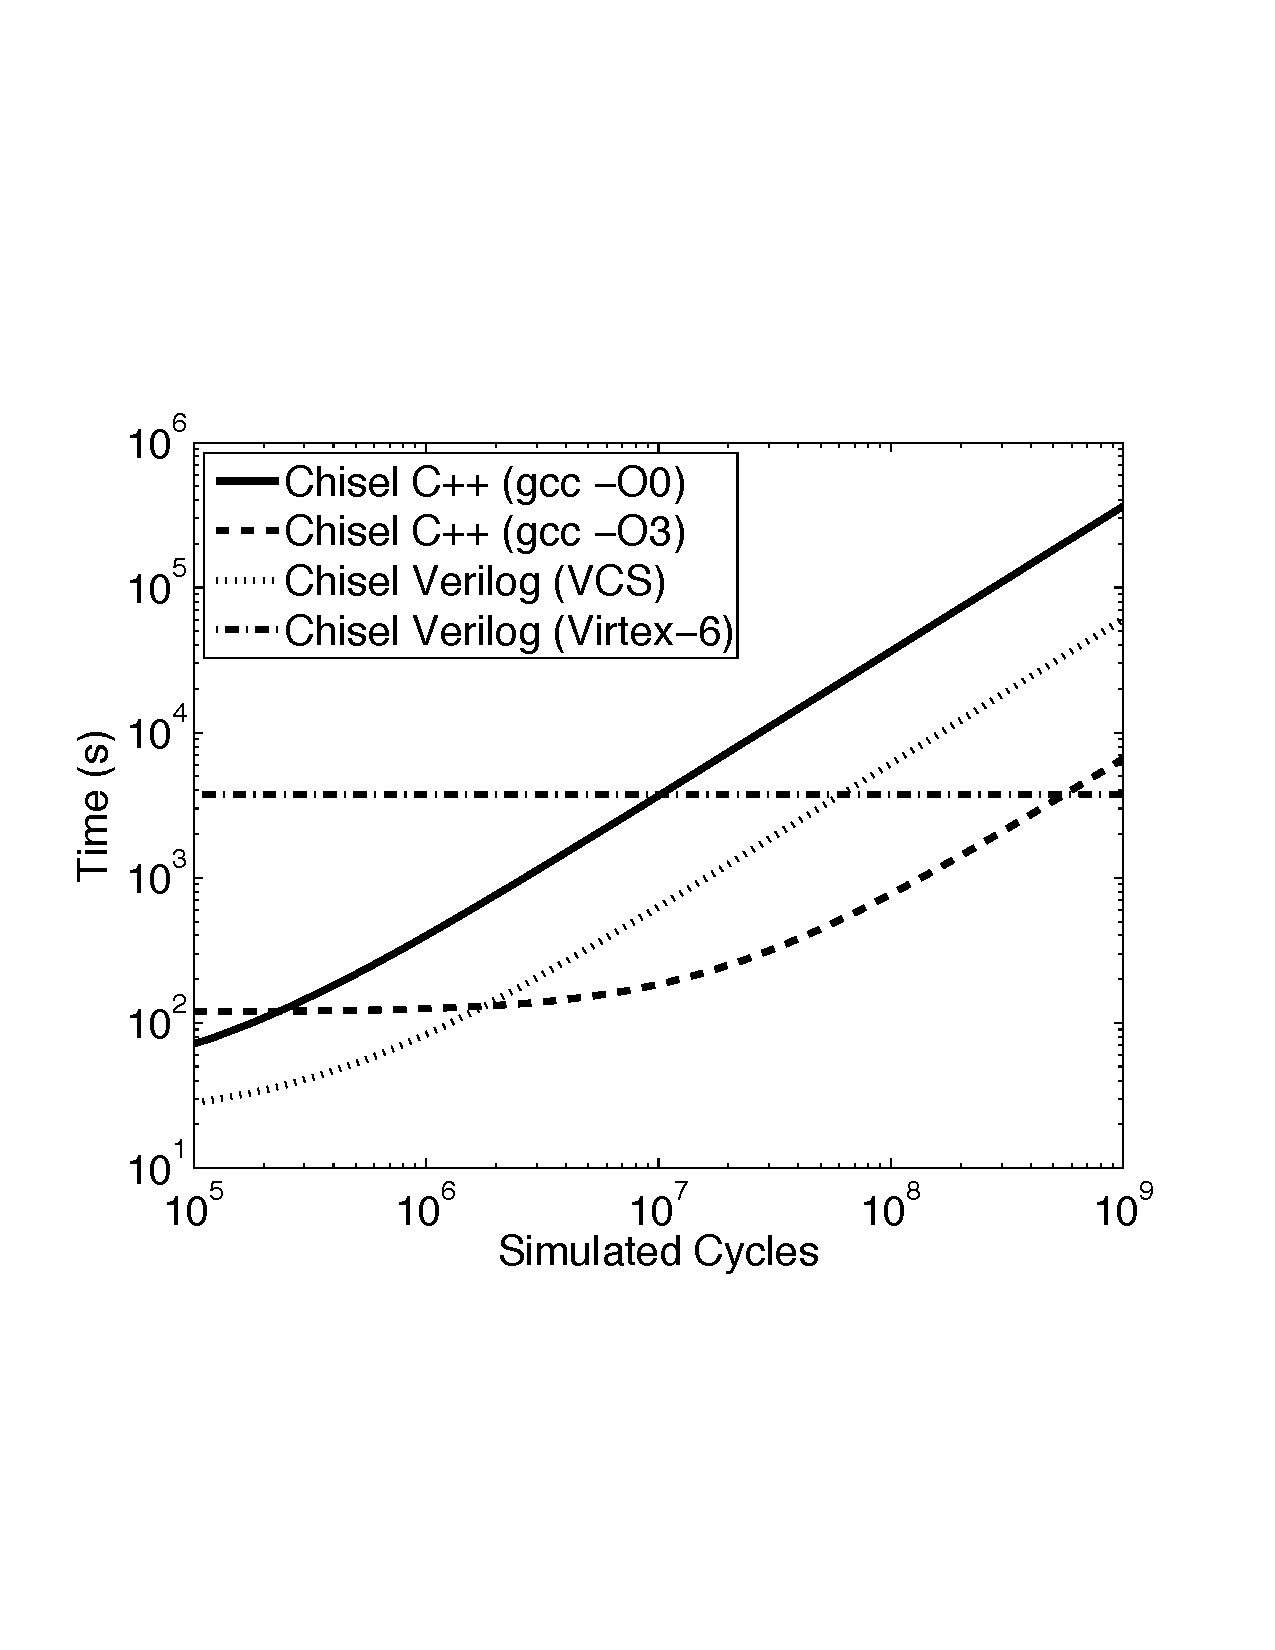
\includegraphics[height=0.9\textheight]{../talks/dac12/figs/perf.pdf}
\end{center}
\end{frame}

\begin{frame}{Chisel Workflow}
\begin{center}
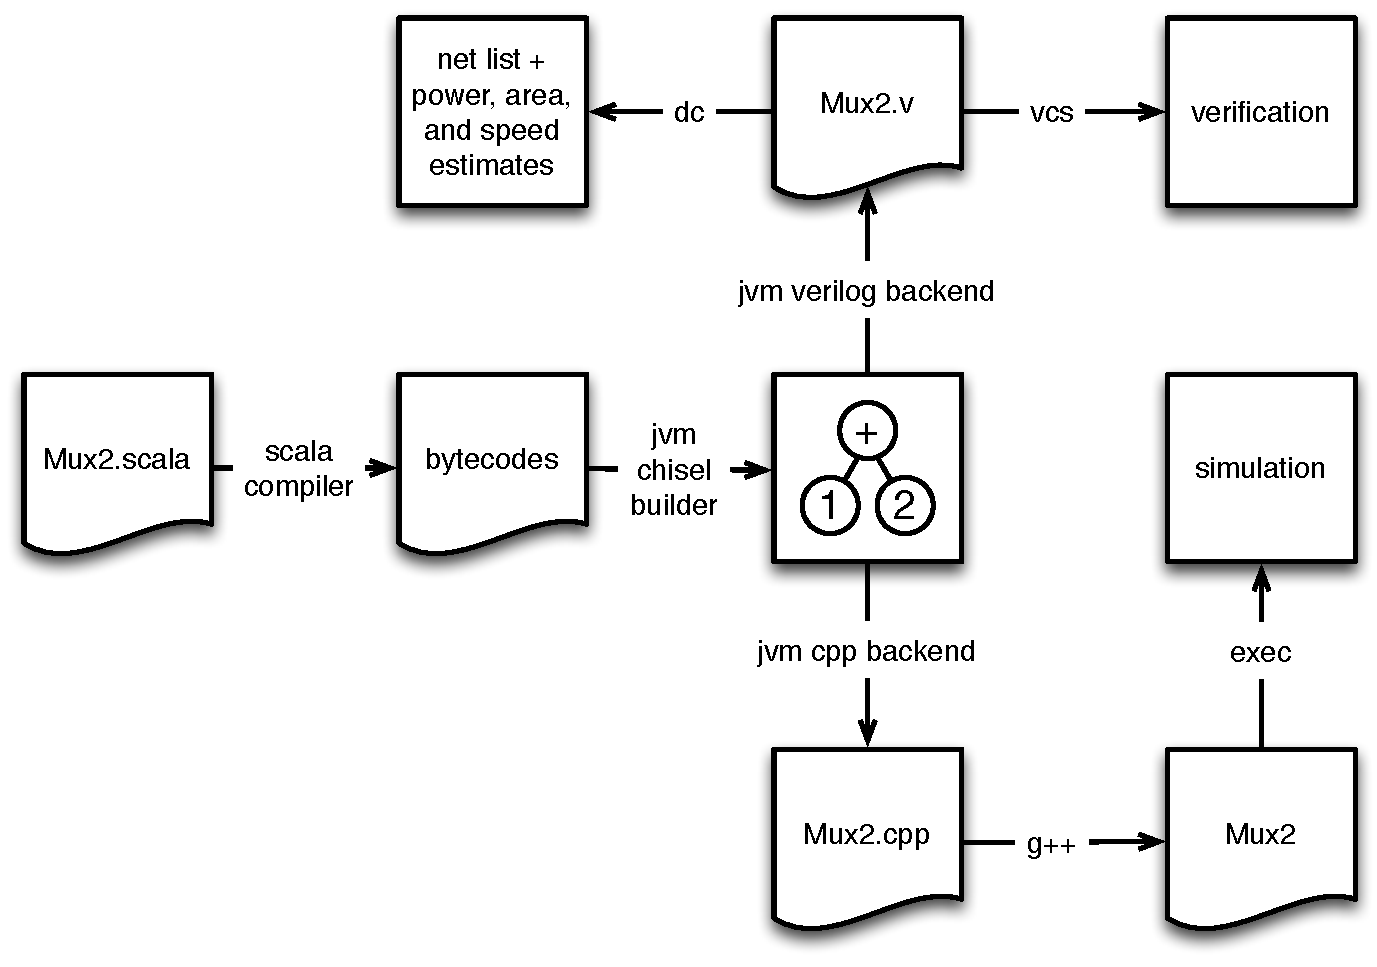
\includegraphics[height=0.9\textheight]{../bootcamp/figs/chisel-workflow.pdf}
\end{center}
\end{frame}

\begin{frame}[fragile]{printf / sprintf}
\begin{itemize}
\item during simulation
\begin{itemize}
\item \verb+printf+ prings the formatted string to the console on rising clock edges
\item \verb+sprintf+ returns the formatted string as a bit vector
\end{itemize}
\item format specifiers are
\begin{itemize}
\item \verb+%b+ -- binary number
\item \verb+%d+ -- decimal number
\item \verb+%x+ -- hexidecimal number
\item \verb+%s+ -- string consisting of a sequence of 8-bit extended ASCII chars
\item \verb+%%+ -- specifies a literal %.
\end{itemize}
\end{itemize}
the following prints the line \verb+"0x4142 16706 AB"+ on cycles when \verb+c+ is true:
\begin{scala}
val x = Bits(0x4142)
val s1 = sprintf("%x %s", x, x);
when (c) { printf("%d %s\n", x, s1); }
\end{scala}
\end{frame}

\begin{frame}[fragile]{assert}
\begin{itemize}
\item simulation time assertions are provided by \verb+assert+ construct
\item if assert arguments false on rising edge then 
\begin{itemize}
\item an error is printed and 
\item simulation terminates
\end{itemize}
\end{itemize}
the following will terminate after 10 clock cycles:
\begin{scala}
val x = Reg(init = UInt(0, 4))
x := x + UInt(1)
assert(x < UInt(10))
\end{scala}
\end{frame}

\begin{frame}{Verilog Debugging}
% \begin{columns}
% \column{0.35\textwidth}
\begin{itemize}
\item produce Verilog from Chisel
\item write tests in Verilog harness
\item use waveform debugger
\end{itemize}
% \column{0.55\textwidth}
% \begin{center}
% 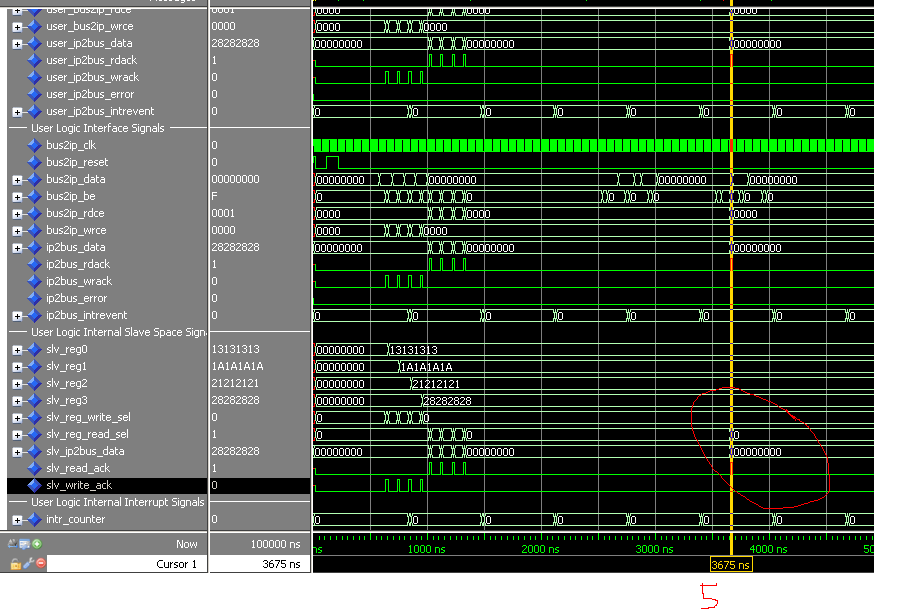
\includegraphics[height=0.7\textheight]{figs/modelsim.png}
% \end{center}
% \end{columns}
\end{frame}

\begin{frame}{Chisel Based Testing Overview}
\begin{columns}
\column{0.55\textwidth}
\begin{itemize}
\item tests written in Chisel
\item Chisel
\begin{itemize}
\item compiles, 
\item runs, and 
\item talks to DUT using pipes
\end{itemize}
\item User
\begin{itemize}
\item sets inputs + get outputs using
\begin{itemize}
\item Chisel data to get nodes and
\item tables from nodes to values
\end{itemize}
\item specifies nodes to trace
\end{itemize}
\end{itemize}

\column{0.35\textwidth}
\begin{center}
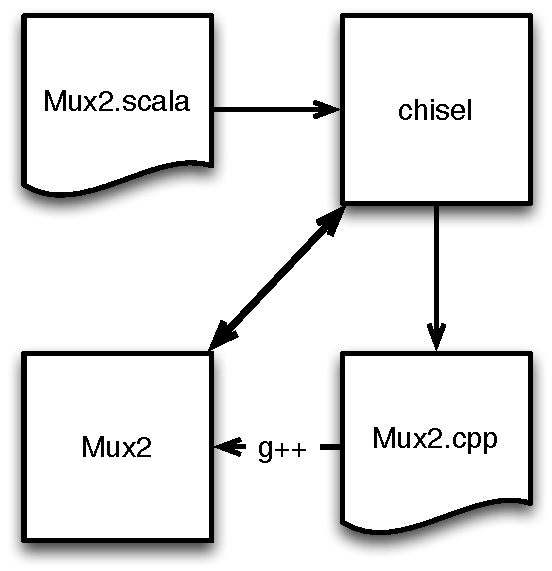
\includegraphics[width=0.9\textwidth]{figs/chisel-testing.pdf}
\end{center}
\end{columns}
\end{frame}

\begin{frame}[fragile]{Chisel Based Testing Details}

\begin{columns}
\column{0.4\textwidth}
{\lstset{basicstyle={\tiny\ttfamily}}
\begin{scala}
package Tutorial
import Chisel._

class Combinational extends Module {
  val io = new Bundle {
    val x = UInt(INPUT, 16)
    val y = UInt(INPUT, 16)
    val z = UInt(OUTPUT, 16) }
  io.z := io.x + io.y
}

class CombinationalTests(c: Combinational) 
    extends Tester(c) {
  val maxInt = 1 << 16
  for (i <- 0 until 10) {
    val x = rnd.nextInt(maxInt)
    val y = rnd.nextInt(maxInt)
    poke(c.io.x, x)
    poke(c.io.y, y)
    step(1)
    expect(c.io.z, (x + y)&(maxInt-1))
  }
}
\end{scala}
}
\column{0.5\textwidth}
{\lstset{basicstyle={\tiny\ttfamily}}
\begin{scala}
class Tester[T <: Module]
  (val c: T, val isTrace: Boolean = true) {
  var ok: Boolean
  val rnd: Random
  def reset(n: Int = 1)
  def poke(data: Bits, x: BigInt)
  def step(n: Int): Int
  def peek(data: Bits): BigInt
  def expect (data: Bits, target: BigInt): Boolean
}
\end{scala}
}
\begin{scriptsize}
users utilize:
\begin{itemize}
\item \code{poke} to set input port and state values,
\item \code{step} to execute the circuit one time unit,
\item \code{peek} to read port and state values, and
\item \code{expect} to compare peeked circuit values to expected arguments.
\end{itemize}
\end{scriptsize}

\begin{center}
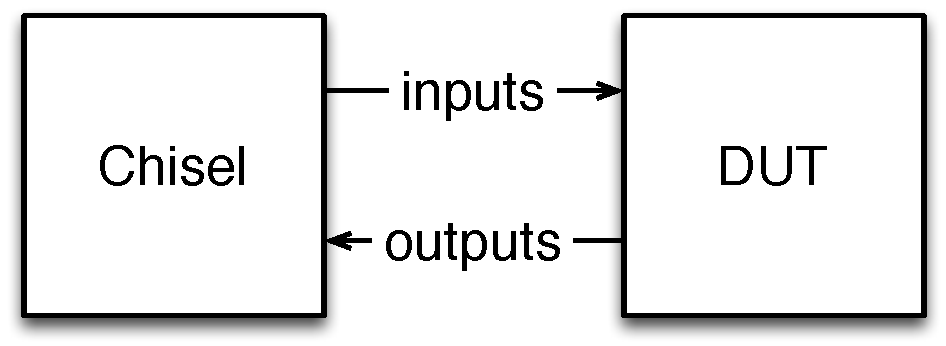
\includegraphics[width=0.8\textwidth]{../tutorial/figs/DUT.pdf}
\end{center}

\end{columns}
\end{frame}

\begin{frame}[fragile]{Binding Tester to Module}

\begin{scala}
object chiselMainTest {
  def apply[T <: Module]
    (args: Array[String], comp: () => T)(
     tester: T => Tester[T]): T
}
\end{scala}

\noindent and used as follows:

\begin{scala}
chiselMainTest(args  ++ Array("--compile", "--test",  "--genHarness"),  
               () => new Combinational()){ 
  c => new CombinationalTests(c) 
}
\end{scala}

\end{frame}

\begin{frame}[fragile]{\code{ChiselMain*} Arguments}
 
\begin{tabular}{ll}
\verb+--targetDir+ & target pathname prefix \\
\verb+--genHarness+ & generate harness file for C++ \\
\verb+--backend v+ & generate verilog \\ 
\verb+--backend c+ & generate C++ (default)\\
\verb+--compile+ & compiles generated C++ \\
\verb+--test+ & generates C++ with test plumbing  \\
\verb+--vcd+ & enable vcd dumping \\
\verb+--debug+ & put all wires in C++ class file \\
\end{tabular}

\end{frame}

\begin{frame}[fragile]{Running Tests Examples}

\begin{scala}
sbt "project tutorial" "run Combinational ... --compile --test --genHarness"
...
PASSED
\end{scala}

or through makefile

\begin{scala}
cd CHISEL/tutorial/emulator
make combinational
...
PASSED
\end{scala}
\end{frame}

\begin{frame}[fragile]{Simple Decoupled Circuits Testing}
\begin{scala}
class GCDTests(c: GCD) extends Tester(c) {
  val (a, b, z) = (64, 48, 16)
  var t = 0
  do {
    val first = if (t == 0) 1 else 0;
    poke(c.io.a, a)
    poke(c.io.b, b)
    poke(c.io.e, first)
    step(1)
    t += 1
  } while (t <= 1 || peek(c.io.v) == 0)
  expect(c.io.z, z)
}
\end{scala}
\end{frame}

\begin{frame}[fragile]{Testing Coprocessor}
\begin{center}
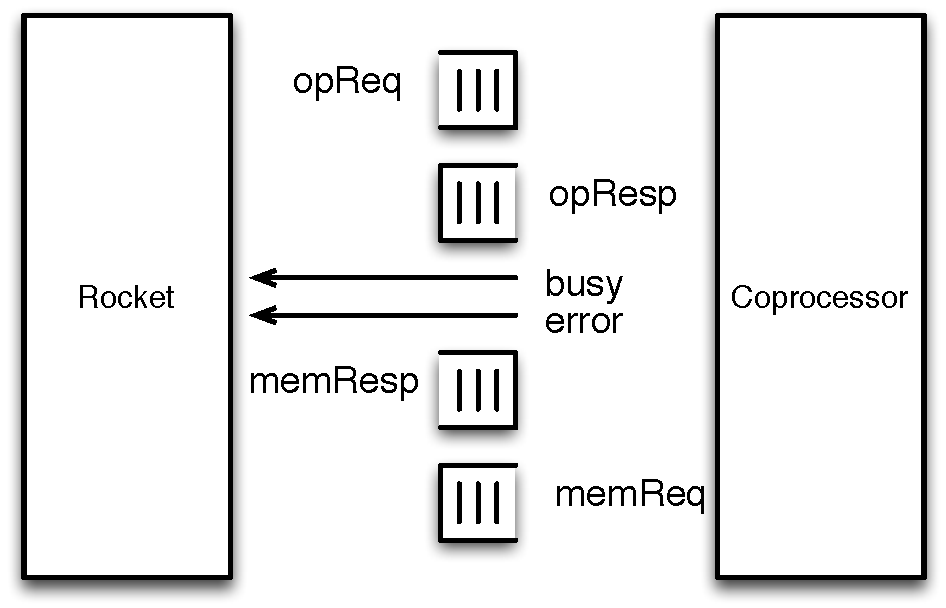
\includegraphics[width=0.8\textwidth]{figs/rocket-coprocessor.pdf}
\end{center}
\end{frame}

\begin{frame}[fragile]{More Powerful Decoupled Circuits}

{\lstset{basicstyle={\scriptsize\ttfamily}}
\begin{scala}
class AdvTester[+T <: Module](val dut: T, val ios: Array[Node])
    extends Tester[T](dut, ios) {

  val preprocessors = new ArrayBuffer[Processable]()

  val postprocessors = new ArrayBuffer[Processable]()

  // like step but does pre and post processing and work
  def takestep(work: => Unit = {}) = ...

  def until(pred: => Boolean, maxCycles: Int = ...)(work: => Unit): Boolean = ...

  def do_until(pred: => Boolean, maxCycles: Int = ...)(work: => Unit): Boolean = ...

  def eventually(pred: => Boolean, maxCycles: Int = ...) = 
    until(pred, maxCycles){ }
}
\end{scala}
}
\vfill 
{\tiny by Stephen Twigg and Eric Love}
\end{frame}

\begin{frame}[fragile]{Sources + Sinks for Testing Decoupled Circuits}
\verb+DecoupledSource+
\begin{itemize}
\item queue from tester to DUT
\item tester enqueues data onto queue
\item handlers moving data from queue to decoupled interface
\item can use \verb+until+ to wait until data shows up on queue
\end{itemize}
\verb+DecoupledSink+
\begin{itemize}
\item queue from DUT to tester
\item tester sees data on queue
\item handlers moving data from decoupled interface to queue
\item can use \verb+until+ to wait until data shows up on queue
\end{itemize}
\end{frame}

\begin{frame}[fragile]{Decoupled Testing Coprocessor}
Imagine testing your coprocessor with AdvTester (instead of rocket core):
\begin{scala}
val commands  = new DecoupledSource(dut.io.cmd, ...)
val responses = new DecoupledSink(dut.io.resp, ...)
...
defTests {
  ...
  commands.inputs.enqueue(TestCmd.setup(0, 1, 10))
  until(!responses.outputs.isEmpty) { } 
  val resp = response.outputs.dequeue()
  assert(resp.data == ..., "test 1 failed: bad response")
  assert(resp.rd == 10, "test 1 failed: bad rd returned")
  ...
}  
\end{scala}
\begin{itemize}
\item memory can also be handled in tester using Scala queues and Scala memory and a process that gets stepped to handle mem requests.
\end{itemize}
\end{frame}

\begin{frame}[fragile]{C++ Simulator}
\begin{itemize}
\item cycle accurate simulator
\begin{itemize}
\item easy way to debug designs
\end{itemize}
\item compile chisel to one C++ class
\begin{itemize}
\item topologically sorts nodes based on dependencies
\end{itemize}
\item simulates using two phases
\begin{itemize}
\item \code{clock\_lo} for combinational
\item \code{clock\_hi} for state updates
\end{itemize}
\item using fast multiword c++ template library
\begin{itemize}
\item now though expand in chisel backend
\item use same representation 
\end{itemize}
\end{itemize}
\end{frame}

\begin{frame}[fragile]{Creating C++ Output}
In order to construct a circuit, 
the user calls \code{chiselMain} from their top level \code{main} function:

\begin{scala}
object chiselMain {
  def apply[T <: Module]
    (args: Array[String], comp: () => T): T
}
\end{scala}

\noindent
which when run creates C++ files named
\code{{\it module\_name}.cpp} and \code{{\it module\_name}.h} in
the directory specified with
\code{--targetDir {\it dir\_name}} argument.

\begin{scala}
chiselMain(Array("--backend", "c", "--targetDir", "../emulator"), 
           () => new GCD())
\end{scala}

\end{frame}

\begin{frame}[fragile]{{\tt dat\_t}}
\begin{scala}
template <int w>
class dat_t {
 public:
  const static int n_words = ((w - 1) / 64) + 1;
  val_t values[n_words];
  inline val_t lo_word ( void ) { return values[0]; }
  ...
}

template <int w> dat_t<w> DAT(val_t value);
template <int w> dat_t<w> LIT(val_t value);

template <int w> std::string dat_to_str (dat_t<w> val);

std::string read_tok(FILE* f);

template <int w> void str_to_dat(std::string str, dat_t<w>& res);
\end{scala}
\end{frame}

\begin{frame}[fragile]{{\tt mod\_t}}
\begin{scala}
class mod_t {
 public:
  std::vector< mod_t* > children;
  virtual void init ( void ) { };
  virtual void clock_lo ( dat_t<1> reset ) { };
  virtual void clock_hi ( dat_t<1> reset ) { };
  virtual void print ( FILE* f ) { };
  virtual bool scan ( FILE* f ) { return true; };
  virtual void dump ( FILE* f, int t ) { };
};
\end{scala}
\end{frame}

\begin{frame}[fragile]{C++ Simulator Outputs}
\begin{itemize}
\item \code{GCD.h} -- the header for the single class
\item \code{GCD.cpp} -- the implementation of the single class
\item \code{GCD-emulator.cpp} -- the harness which cycles the design
\item \code{GCD.vcd} -- produced when running design with vcd output
\end{itemize}
\end{frame}

\begin{frame}[fragile]{GCD.h}
\begin{scala}
#include "emulator.h"

class GCD_t : public mod_t {
 public:
  dat_t<1> GCD__io_v;
  dat_t<16> GCD__io_b;
  dat_t<1> GCD__io_e;
  dat_t<16> GCD__y;
  dat_t<16> GCD__y_shadow;
  dat_t<16> GCD__io_a;
  dat_t<16> GCD__x;
  dat_t<16> GCD__x_shadow;
  dat_t<16> GCD__io_z;

  void init ( bool rand_init = false );
  void clock_lo ( dat_t<1> reset );
  void clock_hi ( dat_t<1> reset );
  void print ( FILE* f );
  bool scan ( FILE* f );
  void dump ( FILE* f, int t );
};
\end{scala}
\end{frame}

\begin{frame}[fragile]{Name Mangling Scheme}
\begin{itemize}
\item chisel object names are mangled to 
\begin{itemize}
\item maintain uniqueness and avoid name conflicts
\item maintain hierarchical membership
\item avoid problems with C++ naming convention
\end{itemize}
\item basic scheme is pathname consisting of
\begin{itemize}
\item Module name first followed by \code{\_\_}
\item hierarchy elements separated with \code{\_}'s in order with
\begin{itemize}
\item numbers for vector elements
\item names for bundle fields
\end{itemize}
\item actual object name last
\end{itemize}
\item examples
\begin{itemize}
\item \code{val io = Bundle\{ val x = UInt(width = 32) \}} produces
\begin{itemize}
\item \code{A\_\_io\_x}
\end{itemize}
\item \code{... Vec.fill(2)\{ Decoupled( Bool() ) \}} produces
\begin{itemize}
\item \code{B\_\_io\_ports\_0\_ready}
\end{itemize}
\end{itemize}
\end{itemize}
\end{frame}

\begin{frame}[fragile]{GCD.cpp}

{\lstset{basicstyle={\tiny\ttfamily}}
\begin{scala}
#include "GCD.h"

void GCD_t::init ( bool rand_init ) {
  { GCD__y.values[0] = rand_init ? rand_val() & 65535 : 0; }
  { GCD__x.values[0] = rand_init ? rand_val() & 65535 : 0; }
}
void GCD_t::clock_lo ( dat_t<1> reset ) {
  val_t T0__w0;
  ...
};
void GCD_t::clock_hi ( dat_t<1> reset ) {
  GCD__y = GCD__y_shadow;
  GCD__x = GCD__x_shadow;
}
void GCD_t::print ( FILE* f ) {
  fprintf(f, "%s", TO_CSTR(GCD__io_z));
  fprintf(f, "%s", " ");
  fprintf(f, "%s", TO_CSTR(GCD__io_v));
  fprintf(f, "\n");
  fflush(f);
}
bool GCD_t::scan ( FILE* f ) {
  str_to_dat(read_tok(f), GCD__io_a);
  str_to_dat(read_tok(f), GCD__io_b);
  str_to_dat(read_tok(f), GCD__io_e);
  return(!feof(f));
}
void GCD_t::dump(FILE *f, int t) {
}
\end{scala}
}
\end{frame}

\begin{frame}[fragile]{GCD-emulator.cpp}
\begin{scala}
#include "GCD.h"
int main (int argc, char* argv[]) {
  GCD_t* c = new GCD_t();
  int lim = (argc > 1) ? atoi(argv[1]) : -1;
  c->init();
  for (int i = 0; i < 5; i++) {
    dat_t<1> reset = LIT<1>(1);
    c->clock_lo(reset);
    c->clock_hi(reset);
  }
  for (int t = 0; lim < 0 || t < lim; t++) {
    dat_t<1> reset = LIT<1>(0);
    if (!c->scan(stdin)) break;
    c->clock_lo(reset);
    c->print(stdout);
    c->clock_hi(reset);
  }
}
\end{scala}
\end{frame}

\begin{frame}[fragile]{VCD Debugging}
\begin{itemize}
\item use \code{--vcd} arg to have simulation produce VCD output
\item run your compiled C++ emulation app for a number of cycles
\begin{itemize}
\item specifying the number of cycles as a first argument
\end{itemize}
\item can view waveforms with
\begin{itemize}
\item \code{vcs} -- commercial
\item GTKWave -- open source
\end{itemize}
\item can hierarchically focus on particular signals
\item can view in a variety of formats
\end{itemize}
\end{frame}

\begin{frame}[fragile]{Manual C++ Testing}
\begin{itemize}
\item test Chisel code by manually 
\begin{itemize}
\item setting circuit inputs directly in your C++ code
\item inserting \code{printf}'s in your C++ code
\end{itemize}
\item in your c++ harness insert calls to
\begin{itemize}
\item \code{str\_to\_dat(read\_tok(f), GCD\_\_io\_a)} to set values
\item \code{TO\_CSTR(GCD\_\_io\_z)} to create string for printing
\end{itemize}
\item in your chisel code
\begin{itemize}
\item wrap nodes with \code{debug} as in \code{debug(io.z)}
\end{itemize}
\item in your \code{chiselMain} 
\begin{itemize}
\item you can add \code{---debug} arg to get everything available in object
\end{itemize}
\end{itemize}
\end{frame}



\begin{frame}[fragile]{Onwards}
\begin{itemize}
\item for simple tests can write test vector files
\item check out Chisel tutorial code
\end{itemize}
\end{frame}

\end{document}
